\documentclass[11pt, a4paper]{article}

\usepackage[utf8]{inputenc}
\usepackage{amsmath, amssymb, amsthm}
\usepackage{geometry}
\geometry{margin=1in}
\usepackage{hyperref}
\usepackage{graphicx}
\usepackage{titlesec}
\usepackage{xcolor}

\hypersetup{
    colorlinks=true,
    linkcolor=blue,
    filecolor=magenta,      
    urlcolor=cyan,
    pdftitle={Innate Working Memory via Memory Residuals},
}

\title{\textbf{Memory Residuals}}
\author{
    \textbf{Yueze Liu} \\
    Independent Researcher  \\
    \href{mailto:yuezel2@illinois.edu}{yuezel2@illinois.edu} 
    \and
    \textbf{Call for Collaboration} \\
    Seeking Academic Partnership
}
\date{\today}

\begin{document}

\maketitle

\begin{abstract}
Modern Large Language Models (LLMs) deployed as conversational agents are constrained by their inability to maintain lifelong, multi-session memory. Current paradigms rely on either concatenating ever-expanding chat histories (leading to context dilution and massive compute overhead) or bolting on external Vector-DB Retrieval-Augmented Generation (RAG) and text summarization systems. Both approaches lack innate cognitive routing—the ability to implicitly choose \textit{what} to remember from the past and \textit{when} to actively recall it. Drawing inspiration from human episodic memory, we propose Memory Residuals. By forcing multi-turn conversation logs through a recurrent, learnable summarizing memory block, we create a dense latent state of user persona and history. Rather than appending this state to the sequence context window, we inject it directly into the depth-wise residual stream, allowing models to seamlessly bypass memory during standard dialogue and sample it heavily during historical callbacks. We further specify the \emph{axis} along which the two-stage update competes: the Stage-2 judge's softmax is taken over the $K$ persistent slots rather than over the $2K$ concatenated inputs, so the competition is between specialists rather than between candidates, and we pair this with a QK-LayerNorm stabiliser that keeps the competition from collapsing to uniform. This position paper outlines the mathematical formulation of Memory Residuals as an elegant replacement for rigid external state-tracking, and calls for collaborative empirical validation.
\end{abstract}

\vspace{0.5cm}

\section{Introduction}
The current trajectory of memory scaling in Transformer-based architectures \cite{vaswani2017attention} fails to address the unique demands of lifelong conversational AI. To give agents persistent memory across thousands of distinct conversational turns, developers either brute-force the context window (expanding sequence length $N$ and suffering from $O(N^2)$ scaling limits), or they rely on rigid, non-differentiable workarounds like text-summarization loops and external Retrieval-Augmented Generation (RAG) databases \cite{lewis2020retrieval}. 

These approaches are fundamentally inefficient. Appending 50 past chat sessions to a system prompt is computationally wasteful for a simple greeting turn, and semantic search often fails to capture evolving implicit user preferences. Human cognition does not perfectly retain raw conversational transcripts, nor does it search a disconnected database to maintain a relationship. Instead:
\begin{enumerate}
    \item \textbf{Human episodic memory is finite and latent} (compressing raw dialogue into dense, high-level semantic abstractions and state).
    \item \textbf{Human memory retrieval is top-down and attention-driven}; we innately route our cognition, bypassing memory for casual conversational filler, and heavily querying past interactions by dynamically weighing them into our active thoughts.
\end{enumerate}

We argue that this dynamic, information-choosing behavior should be baked natively into the architecture. In this paper, we propose a mechanism that merges finite latent space compression with recent advancements in depth-wise attention routing \cite{du2026attention}, creating a persistent, differentiable memory state for multi-session AI.

\section{The Core Paradigm: Memory Residuals}

\begin{figure*}[t]
    \centering
    \includegraphics[width=0.92\textwidth]{1.png}
    
    \caption{\textbf{From Depth-Wise Routing to Persistent Memory.}
    Attention Residuals enable depth-wise competition between intermediate representations, allowing each layer to dynamically route information from prior layers instead of relying on uniform residual addition. Memory Residuals extend this routing view by registering long-term memory as an additional source in the same pool. Each layer can therefore decide whether to use current-session computation or cross-session memory, unifying local reasoning and historical recall under one attention mechanism.}
    \label{fig:unified_memory}
\end{figure*}


We introduce \textbf{Memory Residuals}, an end-to-end differentiable working memory mechanism. It operates by breaking down lifelong conversational tracking into two key architectural advances: the recurrent, incremental construction of a latent episodic memory block, and the dynamic, single-pass querying of that block via the model's internal residual stream.

\subsection{Key Advance 1: Recurrent Updates via Two-Stage QKV Competition}
A naive approach to memory compression might attempt to attend over all historical tokens at once, but this recreates the very $O(N^2)$ context limits we seek to avoid. Furthermore, compressing thousands of conversational turns into a fixed latent bottleneck risks catastrophic forgetting, where conversational filler from a new session overwrites critical persona data established sessions ago.

To resolve this, we formulate the episodic memory block as an incrementally updated matrix $M_{\text{c}} \in \mathbb{R}^{K \times d}$ (where $K$ is a small, fixed number of latent vectors, e.g., 128, and $d$ is the hidden dimension). We update this state using a \textbf{Two-Stage QKV Pipeline}, separating the tasks of information \textit{extraction} and information \textit{judgment}.

Let $M_{\text{c}}^{t-1} \in \mathbb{R}^{K \times d}$ be the persistent latent memory state prior to session $t$, and let $C_t \in \mathbb{R}^{N_t \times d}$ be the raw tokens of the newly completed session.

\paragraph{Stage 1: The Extraction Layer (Compression)}
First, we compress the local session into a dense candidate state $E_t \in \mathbb{R}^{K \times d}$. Using a set of fixed, learnable extraction queries $M_{\text{in}}$, the model pulls only the salient features from the raw session tokens:
\begin{equation}
    E_t = \text{Softmax}\left(\frac{M_{\text{in}} W_Q^{\text{ext}} (C_t W_K^{\text{ext}})^\top}{\sqrt{d}}\right) C_t W_V^{\text{ext}}
\end{equation}

\begin{figure}[t]
    \centering
    \begin{minipage}[t]{0.42\textwidth}
        \centering
        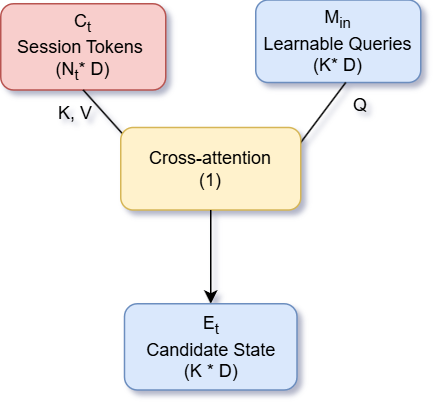
\includegraphics[width=\linewidth]{extraction.png}
    \end{minipage}\hfill
    \begin{minipage}[t]{0.54\textwidth}
        \centering
        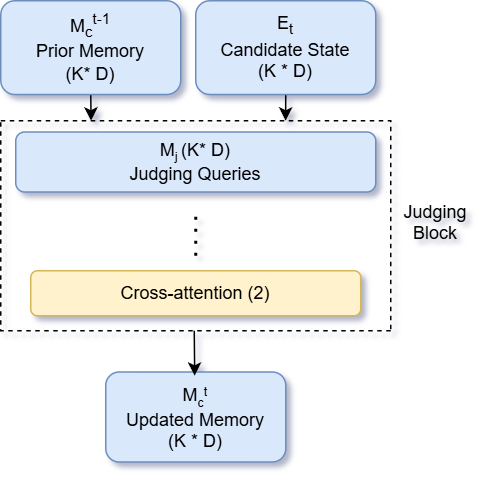
\includegraphics[width=\linewidth]{judging.png}
    \end{minipage}
    \caption{\textbf{Two-stage memory update pipeline.} \textbf{Left:} The extraction block compresses the finished session $C_t$ into a fixed-width candidate state $E_t$ using learnable extraction queries $M_{\text{in}}$. \textbf{Right:} The judging block compares the prior memory $M_{\text{c}}^{t-1}$ against the candidate state $E_t$ using learnable judging queries $M_{\text{judge}}$, producing the updated memory $M_{\text{c}}^t$.}
    \label{fig:two_stage_memory_update}
\end{figure}

\paragraph{Stage 2: The Judging Layer (QKV Competition)}
We now possess two identically sized latent matrices representing the old knowledge ($M_{\text{c}}^{t-1}$) and the newly extracted candidate knowledge ($E_t$). We concatenate them into a combined judgment pool $P_{\text{judge}} =[M_{\text{c}}^{t-1} \parallel E_t] \in \mathbb{R}^{2K \times d}$.

To update the memory, we employ a second cross-attention block governed by a distinct set of persistent, learnable judging queries $M_{\text{judge}} \in \mathbb{R}^{K \times d}$. These queries evaluate the combined pool:
\begin{equation}
    M_{\text{c}}^{t} = \text{Softmax}\left(\frac{M_{\text{judge}} W_Q^{\text{judge}} (P_{\text{judge}} W_K^{\text{judge}})^\top}{\sqrt{d}}\right) P_{\text{judge}} W_V^{\text{judge}}
\end{equation}

\textit{The Forgetting Defense Insight:} Because the Softmax is computed across the $2K$ dimension, the old memory and the new candidate memory are forced into a zero-sum semantic competition. If the new session $C_t$ contains only mundane conversational filler, $E_t$ will lack predictive semantic value. The Judging Queries will recognize this and shift their attention distribution heavily onto the keys of $M_{\text{c}}^{t-1}$, effectively routing the old memory untouched into the next state. Conversely, if $E_t$ contains a critical state-change, the queries will strongly attend to the new representation, implicitly overwriting outdated information.

Figure~\ref{fig:two_stage_memory_update} makes the separation of roles explicit: extraction is responsible for distilling information out of the raw token stream, while judging is responsible for deciding whether the distilled candidate deserves to modify the persistent memory at all.

\subsubsection{On Extraction Depth: Multi-Layer Distillation as an Ablation Axis}
\label{sec:extraction_depth}

Equation~1 assumes that a single cross-attention pass over $C_t$ is sufficient to distill the session's salient semantic content into a $K$-slot candidate. In practice, deciding \textit{what to extract} from a raw conversation of hundreds of tokens is a highly non-linear task: a throwaway mention of "my sister" early in the session may only surface as meaningful after composing it with later turns of the same session. The judging step that follows operates on a $2K$-slot pool and is therefore already a low-bandwidth decision; the capacity we want is in the distillation that \emph{feeds} that decision.

We therefore identify \textbf{extraction depth} $L_E$ as a primary ablation axis, replacing Eq.~1 with a Perceiver-style refinement stack in which the latent state iteratively re-queries the raw session:

\begin{equation}
    E^{(0)} = \text{CrossAttn}^{(0)}\!\left(M_{\text{in}},\; C_t\right) \in \mathbb{R}^{K \times d}
\end{equation}
\begin{equation}
    E^{(\ell)} = E^{(\ell-1)} + \text{CrossAttn}^{(\ell)}\!\left(E^{(\ell-1)},\; C_t\right) \in \mathbb{R}^{K \times d}, \quad \ell = 1, \dots, L_E
\end{equation}

The final candidate $M_{\text{new}} := E^{(L_E)}$ replaces $E_t$ in the judging step of Eq.~2, which remains a single zero-sum competition:
\begin{equation}
    M_{\text{c}}^{t} = \text{Softmax}\!\left(\frac{M_{\text{judge}} W_Q^{\text{judge}} \left(P_{\text{judge}} W_K^{\text{judge}}\right)^\top}{\sqrt{d}}\right) P_{\text{judge}} W_V^{\text{judge}}, \quad P_{\text{judge}} = \left[M_{\text{c}}^{t-1} \parallel M_{\text{new}}\right]
\end{equation}

Because every intermediate state in the refinement lives in $\mathbb{R}^{K \times d}$, the residual in Eq.~4 is well-typed and $L_E = 0$ trivially recovers the single-layer baseline. Deeper stacks ($L_E = 2\text{--}8$) provide non-linear refinement capacity for multi-hop extraction, but must be empirically justified against the risk of overfitting to training-distribution dialogue patterns.

\subsubsection{The Competition Axis: Specialists, Not Candidates}
\label{sec:competition_axis}

Equation~2 / Eq.~5 specifies the semantic competition that drives the recurrent update, but it leaves one architectural choice unstated: \emph{which axis} the Stage-2 softmax is taken over. The form written above takes the softmax over the $2K$ inputs of $P_{\text{judge}}$. For each judging query $M_{\text{judge}}[k]$, attention mass sums to one over the $2K$ rows of $P_{\text{judge}}$; different judging queries compete with nothing --- they independently average over the same input pool. At initialisation the judging queries are random projections of identical magnitude, so every judging query tends to the same content-blind average over $P_{\text{judge}}$, and the gradient of the LM-side loss has no structural pressure to break this symmetry: \emph{any} permutation of the $K$ rows of $M_{\text{judge}}$ leaves the judge's aggregate output invariant. The model is free to settle at a symmetric uniform fixed point in which all $K$ slots hold the same averaged content, and the ``zero-sum'' framing of the competition is vacuous because the competition is between inputs, not between slots.

We therefore specify that the competition is between \emph{specialists} (the $K$ persistent slots), not between \emph{candidates} (the $2K$ input rows). Concretely, the Stage-2 judge's softmax is taken over the slot axis of dimension $K$, so that each input row of $P_{\text{judge}}$ contributes total mass one split across the $K$ slots:
\begin{equation}
    A \;=\; \underset{k \in [K]}{\mathrm{Softmax}}\!\left(\frac{\hat{M}_{\text{judge}}\, W_Q^{\text{judge}}\, \bigl(\hat{P}_{\text{judge}}\, W_K^{\text{judge}}\bigr)^\top}{\sqrt{d}}\right) \in \mathbb{R}^{K \times 2K},
    \label{eq:slot_axis_softmax}
\end{equation}
\begin{equation}
    M_{\text{c}}^{t}[k] \;=\; \frac{\sum_{i=1}^{2K} A[k, i]\, (P_{\text{judge}} W_V^{\text{judge}})[i]}{\sum_{i=1}^{2K} A[k, i] + \varepsilon},
    \label{eq:slot_axis_update}
\end{equation}
where $\hat{M}_{\text{judge}}, \hat{P}_{\text{judge}}$ are RMSNormed inputs to the slot and input streams respectively and $\varepsilon$ is a small numerical stabiliser. Because the softmax normalises along the slot axis, two slots with near-identical query projections share each input row's total unit mass; any drift of one slot's projection \emph{must} be compensated by the other losing mass on the same inputs. Slots therefore have a structural incentive to tile $P_{\text{judge}}$ into disjoint specialist subsets, and the symmetric uniform configuration is no longer a fixed point of the gradient update. This restructuring is the object-centric slot-attention primitive of \cite{locatello2020slot}, repurposed here as the Stage-2 judge; we retain the two-stage pipeline of Eq.~1--2 unchanged, and the recurrent update $M_{\text{c}}^{t} = \mathrm{LayerNorm}(M_{\text{c}}^{t-1} + \Delta_{M_\text{c}}^{t})$ is computed against Eq.~\ref{eq:slot_axis_update}'s output through a standard per-slot gated cell so that the update is recurrent rather than overwriting.

\paragraph{Stabilising the competition: QK-LayerNorm.} Even with the slot-axis softmax, the judge is a single attention layer whose logits decay exponentially fast with the spectral norm of $W_Q^{\text{judge}}$ and $W_K^{\text{judge}}$ \cite{zhai2023sigmareparam}. Under small step-size gradient descent on the LM objective, the spectral norms drift towards small values, and the slot-axis softmax' per-input-row distribution drifts back towards uniform across slots --- the entropy-collapse pathology of \cite{zhai2023sigmareparam} reasserted on the slot axis. We therefore apply post-projection RMSNorm to the judge's query and key images before the inner product,
\begin{equation}
    Q^{\text{judge}} = \mathrm{RMSNorm}\bigl(\hat{M}_{\text{judge}}\, W_Q^{\text{judge}}\bigr),
    \quad
    K^{\text{judge}} = \mathrm{RMSNorm}\bigl(\hat{P}_{\text{judge}}\, W_K^{\text{judge}}\bigr),
    \label{eq:qk_layernorm}
\end{equation}
so that the attention logits are $d^{-1/2}\langle Q^{\text{judge}}, K^{\text{judge}}\rangle$ with $Q^{\text{judge}}, K^{\text{judge}}$ of unit per-row RMS. The magnitude of attention logits is then decoupled from the spectral norm of $W_Q^{\text{judge}}, W_K^{\text{judge}}$, so the slot-axis softmax retains the freedom to sharpen without the LM objective having to carefully tune the spectral norms of two projections whose job is semantically independent of logit scale. QK-LayerNorm has become the standard attention-entropy-collapse stabiliser in recent large-scale Transformers (used in Qwen, Gemma, and DeepSeek-V3); its application here is only incrementally novel in that it is applied to the judge whose logits otherwise drive the zero-sum semantic competition.

\paragraph{Net effect on the two-stage pipeline.} The forward of the extraction stage (Eq.~1 / Eq.~3--4) is unchanged; the only architectural delta is the Stage-2 judge, which replaces the input-axis softmax of Eq.~2 / Eq.~5 with the QK-LayerNormed slot-axis update of Eq.~\ref{eq:slot_axis_softmax}--\ref{eq:qk_layernorm}. Because the rest of the primitive --- the extraction stack, the readout $m^t$, and the depth-wise router --- attends against $M_{\text{c}}^{t}$ as a $K\!\times\!d$ matrix, the slot-axis judge is a drop-in replacement with no downstream re-plumbing required.

\subsection{Key Advance 2: Implicit Retrieval via the Depth-Wise Residual Stream}

Our second advance defines how the active model queries the persistent state $M_{\text{c}}^t$ during a live conversation. Treating memory retrieval as a standard token-level attention operation over a concatenated pool would reintroduce an $O((N+K)^2)$ bottleneck. To avoid sequence-length bloat, we register the episodic memory block directly into the model's \emph{depth-wise} residual stream, utilizing the principles of Attention Residuals \cite{du2026attention}.

\paragraph{Reading Memory as a Source Stream.}
Depth-wise routing frameworks treat each layer's output as a source tensor of shape $S \times d$: one $d$-dimensional vector per token position in the current session. To interface seamlessly with this structure---and to let each position in the current session retrieve the memory slot most relevant to its local context---we read out from the $K$-row memory matrix $M_{\text{c}}^t$ via a cross-attention whose queries are the current session's token embeddings $X \in \mathbb{R}^{S \times d}$:

\begin{equation}
    m^t = \text{Softmax}\!\left(\frac{X W_Q^{\text{read}} (M_{\text{c}}^t W_K^{\text{read}})^\top}{\sqrt{d}}\right) M_{\text{c}}^t W_V^{\text{read}} \in \mathbb{R}^{S \times d}
\end{equation}

Each position $s$ attends over the $K$ memory slots independently, so the readout is inherently query-dependent: tokens discussing a family conflict route mass onto slots encoding family context, while tokens about dinner plans attend elsewhere. Because $m^t$ has exactly the shape of a standard attention layer's output, it drops directly into the depth-wise routing pool described below without any special-casing.

\paragraph{Registering Memory as the Foundational Layer.}
Let a model have $L$ layers. In a depth-wise attention system, layer outputs act as source tensors $v_1, \ldots, v_{L-1}$ (each of shape $S \times d$) that can be queried by subsequent layers. We introduce the per-position memory readout as the foundational source at index 0:

\begin{equation}
    v_0 := m^t \quad \in \mathbb{R}^{S \times d}
\end{equation}

The input to any downstream layer $l$ is computed as a depth-wise softmax attention over all preceding sources, \textit{including} the episodic memory:

\begin{equation}
    h_l = \sum_{i=0}^{l-1} \alpha_{i \to l} \cdot v_i,
    \qquad
    \alpha_{i \to l} = \frac{\phi(w_l,\, k_i)}{\sum_{j=0}^{l-1} \phi(w_l,\, k_j)}
    \label{eq:memres_attn}
\end{equation}

where $\phi(q, k) = \exp\!\left(q^\top \operatorname{RMSNorm}(k)\right)$ and $w_l \in \mathbb{R}^d$ is a learned pseudo-query for layer $l$. The keys are defined simply as:

\begin{equation}
    k_i = v_i =
    \begin{cases}
        m^t & i = 0 \quad \text{(episodic memory)} \\
        f_i(h_i) & 1 \leq i \leq l-1 \quad \text{(layer outputs)}
    \end{cases}
\end{equation}

\paragraph{Implicit Cognitive Routing.}
By integrating memory directly into the layer-to-layer residual stream, the model gains the ability to implicitly control memory recall without gating heuristics. During a content-rich conversational turn, the recent hidden states ($v_1, \ldots, v_{l-1}$) will naturally dominate the softmax competition, suppressing $\alpha_{0 \to l}$ and bypassing historical memory. Conversely, during a sparse or ambiguous turn (e.g., a bare pronoun callback like "Did you ask her yet?"), the absence of dominant local features allows the memory source $v_0$ to attract higher attention weight. This structurally replicates the selective, top-down nature of human cognitive retrieval.

\section{Distinction from Existing Paradigms}
While our approach shares philosophical DNA with several recent works, it uniquely resolves the limitations of modern agentic workflows:
\begin{itemize}
    \item \textbf{Versus Standard RAG and MemGPT:} Memory Residuals are entirely end-to-end differentiable. The model learns \textit{how} to encode implicit user preferences based on backpropagated loss, eliminating the need for rigid vector databases and lossy text-summarization prompts.
    \item \textbf{Versus Attention Residuals \cite{du2026attention}:} While recent work replaces uniform depth-wise addition with a softmax attention mechanism over \textit{internal} layer outputs, Memory Residuals expand this paradigm to the \textit{external} temporal domain. By injecting a per-position cross-session readout $m^t$ as the foundational source ($v_0$), we bridge the gap between intra-session depth routing and lifelong memory retrieval while preserving the query-dependent selectivity of standard attention.
    \item \textbf{Versus Perceiver IO \cite{jaegle2021perceiver}:} While Perceiver uses cross-attention bottlenecks to handle large inputs, Memory Residuals embed this bottleneck specifically as a \textit{softmax-weighted depth source}, allowing context-dependent querying on a turn-by-turn basis.
    \item \textbf{Versus Recurrent Memory Transformer (RMT) \cite{bulatov2022recurrent}:} Models like RMT prepend memory embeddings directly to the context window. Memory Residuals remove memory from the standard $O(N^2)$ sequence entirely, isolating it in the orthogonal depth-wise routing pool.
\end{itemize}

\section{Empirical Roadmap: Training via Episodic TV Scripts}
A significant bottleneck in lifelong conversational AI research is the lack of high-quality, long-horizon dialogue data exhibiting true implicit memory recall. Synthetic datasets lack emotional depth, and real-world assistant logs are frequently restricted by privacy constraints.

To empirically validate Memory Residuals, we propose utilizing \textbf{Episodic TV Show Transcripts} (e.g., sitcoms and long-form dramas) as our primary training and benchmarking corpus. TV scripts represent the gold standard of multi-session human dialogue. They are defined by stable character personas, long contexts, and explicitly scripted "callbacks" (e.g., a thematic reference in Season 3 that relies entirely on a brief interaction from Season 1).

By feeding transcripts episode-by-episode into the model and updating $M_{\text{c}}$ sequentially, we can evaluate the model's ability to execute a semantic callback across massive token spans. Successfully retrieving the context of a Season 1 event during a Season 3 generation—while ignoring hundreds of intervening episodes of casual filler—will empirically prove that the Memory Residuals mechanism accurately mimics human selective recall.

\section{Conclusion and Call for Collaboration}
The Memory Residuals architecture presents a mathematically elegant solution to the exploding context constraints and rigid external memory systems of multi-turn AI agents. By combining a recurrent, competition-driven episodic memory block with depth-wise residual routing---and by specifying that the Stage-2 competition is between persistent slots, not between candidate inputs, and stabilised by QK-LayerNorm so it cannot silently collapse to uniform---we provide a blueprint for models that innately understand when to ignore the past, and when to actively retrieve it.

I have established the theoretical framework and foundational mathematics for this approach. I am currently seeking an academic laboratory or partner with compute resources to collaborate on scaling this architecture. Future work will execute the TV-script training curriculum to validate the activation of the memory attention weights ($\alpha$), with the ultimate goal of co-authoring a formal publication for upcoming AI conferences (e.g., NeurIPS, ICLR).

% ==========================================
% REFERENCES
% ==========================================
\begin{thebibliography}{99}

\bibitem{vaswani2017attention}
Vaswani, A., Shazeer, N., Parmar, N., Uszkoreit, J., Jones, L., Gomez, A. N., Kaiser, \L{}., \& Polosukhin, I. (2017). 
\textit{Attention is all you need}. 
Advances in Neural Information Processing Systems, 30.

\bibitem{liu2024lost}
Liu, N. F., Lin, K., Hewitt, J., Paranjape, A., Bevilacqua, M., Petroni, F., \& Liang, P. (2024). 
\textit{Lost in the middle: How language models use long contexts}. 
Transactions of the Association for Computational Linguistics, 12, 157--173.

\bibitem{lewis2020retrieval}
Lewis, P., Perez, E., Piktus, A., Petroni, F., Karpukhin, V., Goyal, N., K\"{u}ttler, H., Lewis, M., Yih, W., Rockt\"{a}schel, T., Riedel, S., \& Kiela, D. (2020). 
\textit{Retrieval-augmented generation for knowledge-intensive NLP tasks}. 
Advances in Neural Information Processing Systems, 33, 9459--9474.

\bibitem{du2026attention}
Kimi Team (Du, Y., et al.). (2026). 
\textit{Attention Residuals}. 
arXiv preprint arXiv:2603.15031.

\bibitem{jaegle2021perceiver}
Jaegle, A., Borgeaud, S., Alayrac, J.-B., Doersch, C., Ionescu, C., Ding, D., Koppula, S., Zoran, D., Brock, A., Shelhamer, E., \& H\'{e}naff, O. (2021). 
\textit{Perceiver IO: A General Architecture for Structured Inputs \& Outputs}. 
International Conference on Learning Representations (ICLR).

\bibitem{bulatov2022recurrent}
Bulatov, A., Kuratov, Y., \& Burtsev, M. S. (2022). 
\textit{Recurrent Memory Transformer}. 
Advances in Neural Information Processing Systems, 35, 11079--11091.

\bibitem{chevalier2023adapting}
Chevalier, A., Wettig, A., Ajith, A., \& Chen, D. (2023). 
\textit{Adapting Language Models to Compress Contexts}. 
Proceedings of the 2023 Conference on Empirical Methods in Natural Language Processing (EMNLP).

\bibitem{locatello2020slot}
Locatello, F., Weissenborn, D., Unterthiner, T., Mahendran, A., Heigold, G., Uszkoreit, J., Dosovitskiy, A., \& Kipf, T. (2020).
\textit{Object-centric learning with slot attention}.
Advances in Neural Information Processing Systems, 33.

\bibitem{zhai2023sigmareparam}
Zhai, S., Likhomanenko, T., Littwin, E., Busbridge, D., Ramapuram, J., Zhang, Y., Gu, J., \& Susskind, J. M. (2023).
\textit{Stabilizing Transformer Training by Preventing Attention Entropy Collapse}.
Proceedings of the 40th International Conference on Machine Learning (ICML).

\end{thebibliography}

\end{document}